\section{Implementation}
\label{section:implementation}

This chapter will discuss the implementation of the mobile version of \gls{see}, starting with the mobile player implementation in section \ref{sec:player}.
Section \ref{sec:player_movement} will give insight on the player movement before section \ref{sec:menu} will discuss the mobile menu.
Next, the implemented player action will be introduced in section \ref{sec:player_actions}.
This chapter will end with pointing out the requirements for an \gls{android} build and how they have been handled.
\subsection{Mobile Player}
\label{sec:player}
In this section the mobile player \gls{prefab} will be discussed. 
\gls{see} is supported on multiple platforms and with each platform having different requirements, each platform needs to be divided.
Therefore, each platform gets its own player \gls{prefab}.
The mobile player prefab for the \gls{android} version of \gls{see} can be seen in figure \ref{fig:prefab}.

\begin{figure}[htb]
    \centering
    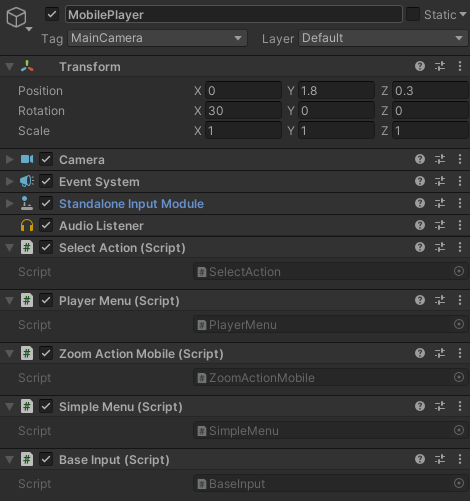
\includegraphics[width=0.8\textwidth]{Implementation/img/mobile_player.png}
    \caption{The mobile player \gls{prefab}}\label{fig:prefab}
\end{figure}

The \gls{prefab} consists of the basic parts provided by \gls{unity} \textit{Camera}, \textit{Event System}, \textit{Standalone Input Module} and \textit{Audio Listener}.
In addition to that the following custom scripts were added.
There is the \textit{SelectAction} and the \textit{ZoomActionMobile} script, which will both be discussed in section \ref{sec:player_actions}, and then there is the \textit{PlayerMenu} script, which creates the right menu based on the player type.
In this case the player type will be \enquote{mobile player} and the menu created (here \textit{SimpleMenu}) will be discussed in section \ref{sec:menu}.

\subsection{Player Movement}
\label{sec:player_movement}
After having created a player, the player also has to be able to move.
Therefore, the \textit{MobilePlayerMovement} script got added.
The script handles the input by the joysticks seen in figure \ref{fig:joystick}.
To fulfill [R2.1] the player will be moved by using the left joystick and the player's perspective will be handled by the right joystick.

\begin{figure}[htb]
    \centering
    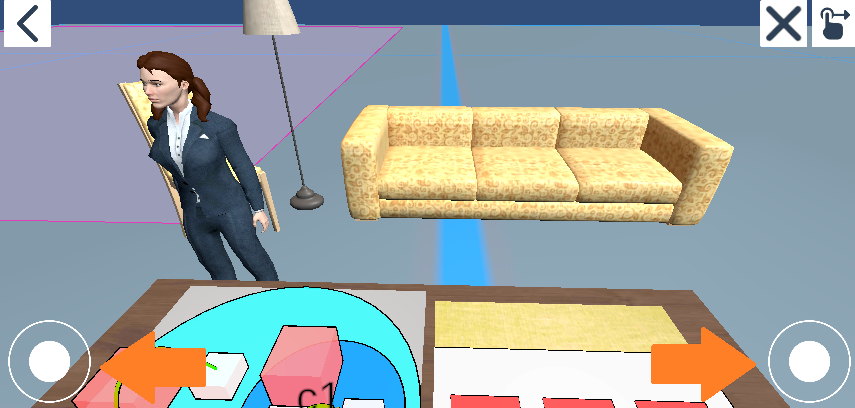
\includegraphics[width=1\textwidth]{Implementation/img/joysticks.png}
    \caption{The joysticks are for moving in the virtual room. The left joystick is for moving the player and the right one is for moving the player's perspective.}\label{fig:joystick}
\end{figure}

For the joystick \glspl{prefab} the \textit{Joystick Pack}\footnote{https://assetstore.unity.com/packages/tools/input-management/joystick-pack-107631\#description (last visited: 17.06.22, 15:21)} \gls{asset} is used.
It contains the design and basic logic for the joysticks.
A joystick returns a horizontal and a vertical value depending on how far the joystick is dragged into a direction.
The left joystick data can then be transformed into player movement as follows:
\begin{enumerate}
    \item Get the horizontal and vertical values from the joysticks
    \item Transform the values into a 3D vector
    \item Combine the values into a velocity vector
    \item Normalize the velocity vector for a smooth transition
    \item Transmit the velocity vector to the player position value
\end{enumerate}

The data of the right joystick shall move the player's perspective, which is implemented as a \gls{unity} camera.
The camera has a pitch angle and a yaw angle as illustrated in figure \ref{fig:camera}.
The angles of the camera will be adjusted with the input from the right joystick. 
For the angles of the player's perspective there is a range from 0° to 360°, after reaching an end of this range the value will be transformed to the other end of the range.
In other words, if the angle becomes higher than 360° it starts at 0° again and if it gets lower than 0°, it can go further down from 360°.
In that way the player's perspective can move a full rotation.
\begin{figure}[htb]
    \centering
    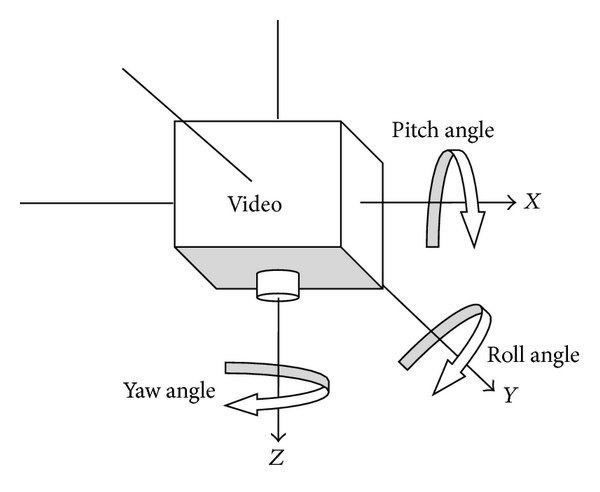
\includegraphics[width=1\textwidth]{Implementation/img/pitch_yaw.jpg}
    \caption{The angles of a camera by \cite{Zhang2014}}\label{fig:camera}
\end{figure}

\subsection{Mobile Menu}
\label{sec:menu}

The mobile menu is essential for the implementation since the input methods of a smartphone in an everyday usage are limited.
The desktop version uses many \glspl{shortcut}, which cannot be used in the mobile version.
These \glspl{shortcut} will be replaced with buttons in the menu to fulfill requirement [R2.2].

\begin{figure}[htb]
    \centering
    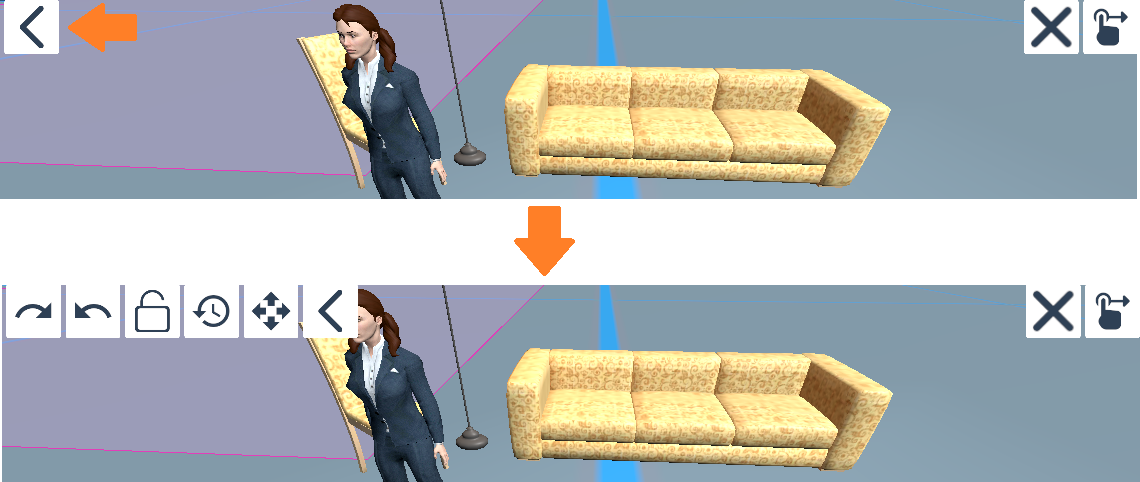
\includegraphics[width=1\textwidth]{Implementation/img/quickmenu.png}
    \caption{The \textit{quickbar} on the left top side of the mobile device. Pressing the button with an orange marked arrow will expand the menu.}\label{fig:quickmenu}
\end{figure}

The menu will be divided into two parts.
The first part, which was named \textit{quickbar} in section \ref{sec:interface}, will be responsible for all interactions that need to be available at all times.
The implemented \textit{quickbar} can be seen in figure \ref{fig:quickmenu}.
By pressing the button on the right end of the \textit{quickbar}, the menu can be expanded and minimized to safe screen space when not needed.
The menu also contains buttons for redoing and undoing actions to fulfill requirement [R8].
In addition, there is a button for a \enquote{locked-mode}.
Unfortunately, the button is just a placeholder since the functionality to lock the players view to a city is not available in the desktop version at this time.
Therefore, requirement [R9] can not be completed at the time of this thesis. 

The other part of the menu can be seen in figure \ref{fig:interaction_menu}.
The menu is placed on the right side of the screen, and it contains all the player interactions.
This part of the menu is slightly more complex since the selected button moves to the top, while the other buttons shall remain their initial order.

\begin{figure}[htb]
    \centering
    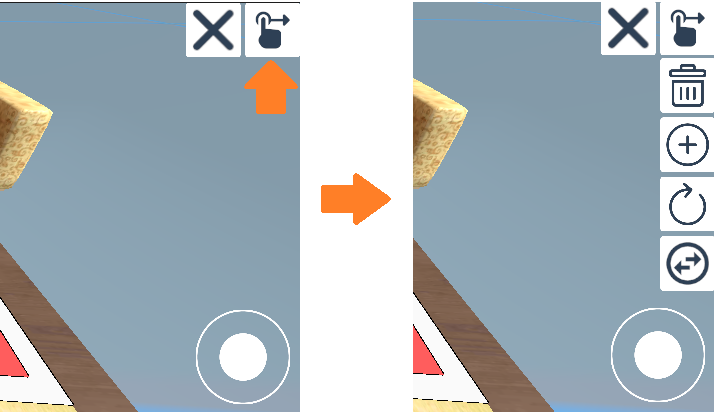
\includegraphics[width=1\textwidth]{Implementation/img/menu.png}
    \caption{The player interaction menu on the right top side of the mobile device. The button on the top right side indicate the active interaction mode. Pressing the same button also expands the menu.}\label{fig:interaction_menu}
\end{figure}

The implementation of the menu on the right is done in the following steps:
\begin{enumerate}
    \item All main buttons get an index
    \item When a button on the far right side gets clicked, the index gets saved
    \item The button group with the selected index get shown on the top right side
    \item All other buttons get disabled
    \item By clicking the button on the top right again, the other main buttons get reactivated 
    \item The order is as follows: selected index → index in ascending order
\end{enumerate} 
This way the selected interaction mode will always be in the top right corner, while the other buttons remain the same order.

\subsection{Player Actions}
\label{sec:player_actions}

One essential part of the implementation are the player actions. 
Almost all interactions a user can make in \gls{see} differ from the interactions in the desktop version.
In the following, the implementation of all mobile player actions will be discussed briefly.

\subsubsection{Zooming}
To fulfill requirement [R2.3], zooming needs to be implemented.
The interaction of zooming in or out of a \gls{city} can be fundamental when working with a large \gls{city} because \glspl{node} become small and especially on a small mobile screen it becomes impossible to interact with those \glspl{node} via touch input. 
Therefore, the user has to zoom in to properly interact with the desired \gls{node}.

Luckily the general zooming function is already implemented in \gls{see}.
The zooming method requires a center point and a scale of how far the \gls{city} shall be zoomed in or out.
Zooming on a touchscreen will be done by dragging two fingers either towards or away from each other as visualized in figure \ref{fig:zooming}.

\begin{figure}[htb]
    \centering
    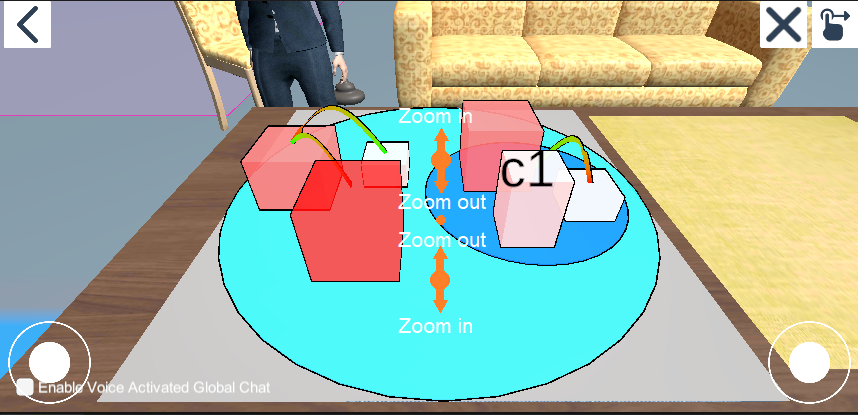
\includegraphics[width=1\textwidth]{Implementation/img/zoom.png}
    \caption{Dragging the two touch points towards each other will zoom out and dragging them away from each other will zoom in.}\label{fig:zooming}
\end{figure}

The implementation of the zooming interaction in done in the following steps: 
\begin{enumerate}
    \item Check if there are two touch inputs on the same \gls{city}. If both inputs are not on the same city, zooming is not wanted and will not be activated.
    \item Compute the center of the two touch inputs
    \item Pass the center and dragging range of the two inputs to the zooming function
\end{enumerate}

Note that the direction of zooming has been inverted in the version used for the evaluation in chapter \ref{section:evaluation}.
This is because of the heavy demand by the subjects to invert the direction of zooming since it felt odd.

\subsubsection{Selecting and Deleting}
The interactions of selecting and deleting a \gls{node} or \gls{plane} are quite similar because the user selects or deletes an object by touching it.
The object get determined by a ray cast from the center of the touch position as discussed in section \ref{sec:ray}.

Since the selecting mode is always enabled except when the delete mode is active, the select button really does nothing apart from ensuring that no other interaction mode is active.
Keeping the selected objects active makes sense for the mobile version because the user cannot hover with a mouse to see the object names.
Therefore, the selection will be kept and not discarded by selecting a different object as in the desktop version.
The deselect button calls the already implemented \textit{UnselectAll} method that empties a list of selected items.

The delete-interaction works as already mentioned just like in the desktop version. 
The only difference is the type of input. 
Other than in the desktop version, the mobile version only supports single deletions and not the deletion of multiple objects at once.
This is due to the limited space for the interactions menu and the results from a multi deletion can also be achieved with the single delete interaction.

The discussed implementation fulfills requirements [R3] and [R4].

\subsubsection{Node Interactions}

The \gls{node} interactions consist of four types.
The active interaction is always highlighted in green as seen in figure \ref{fig:node}
\begin{figure}[htb]
    \centering
    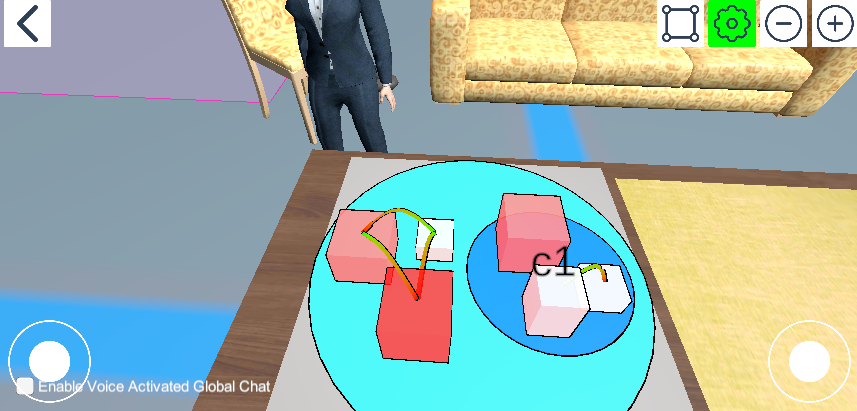
\includegraphics[width=1\textwidth]{Implementation/img/node.png}
    \caption{The \gls{node} interactions menu. The active \gls{node} interaction has a green button}\label{fig:node}
\end{figure}

The circled plus button stands for adding a \gls{node}.
Adding \glspl{node} is implemented in the following steps:
\begin{enumerate}
    \item Check if the device is an \gls{android} with a preprocessor tag
    \item Check if there is exactly one touch input
    \item Cast a ray and check if the collided object is of the type \enquote{Node} (\gls{see} does not distinguish between \gls{plane} and \gls{node} as a type)
    \item Create a \gls{node} at that position with the already implemented \textit{AddChild} method of the class \textit{GameNodeAdder}
\end{enumerate}

The circled minus button is for adding an \gls{edge}.
The implementation is quite similar to the one for adding \glspl{node}.
In this case however the first and second \gls{gameObject} of type \enquote{\gls{node}} will be saved.
After there are two \glspl{gameObject}, an \gls{edge} between those objects will be created.

Next in line is the gear button, which can be used for editing \glspl{node}.
The implementation here is almost the same as for the desktop version.
A \gls{node} or a \gls{plane} can be selected by touch and a window will open.
In that window attributes like the name can be changed.
Different from the desktop version is that a virtual keyboard will pop up to let the user type in a new name for example.

Last but not least, there is the interaction of scaling a \gls{node} left.
The implementation here was largely adopted from the desktop version, except again the input type is via touch.
In addition to that, the dots that can be selected and dragged are larger in the mobile version (see figure \ref{fig:scale}), because otherwise it would be hard to hit them with a touch input.

\begin{figure}[htb]
    \centering
    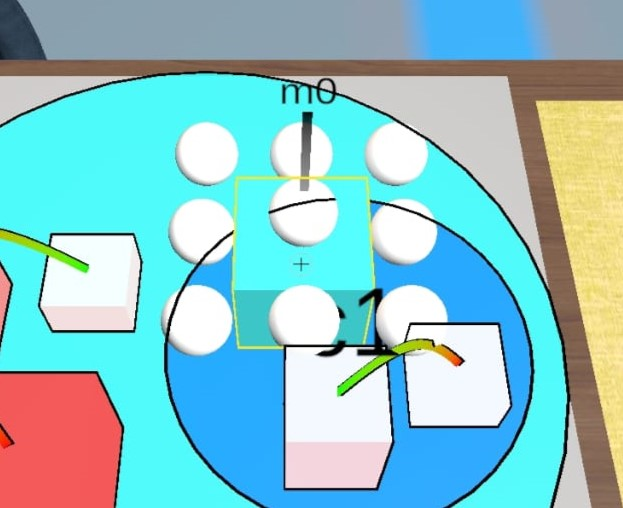
\includegraphics[width=0.7\textwidth]{Implementation/img/scale.jpeg}
    \caption{The \gls{node} interactions menu. The active \gls{node} interaction has a green button}\label{fig:scale}
\end{figure}

The listed implementations of the \gls{node} interactions fulfill the requirements of [R5].

\subsubsection{Rotating}
To fulfil the requirements of [R6], rotating has to be adapted to the mobile version of \gls{see}.
The user can rotate the city either freely or in eight predefined steps.
Figure \ref{fig:rotate} shows a rotation in those eight predefined steps.
As it can be seen the \enquote{8} button is green which means that it is active.
The user can drag from a certain point on the \gls{city} towards a direction the \gls{city} shall be rotated to.

\begin{figure}[htb]
    \centering
    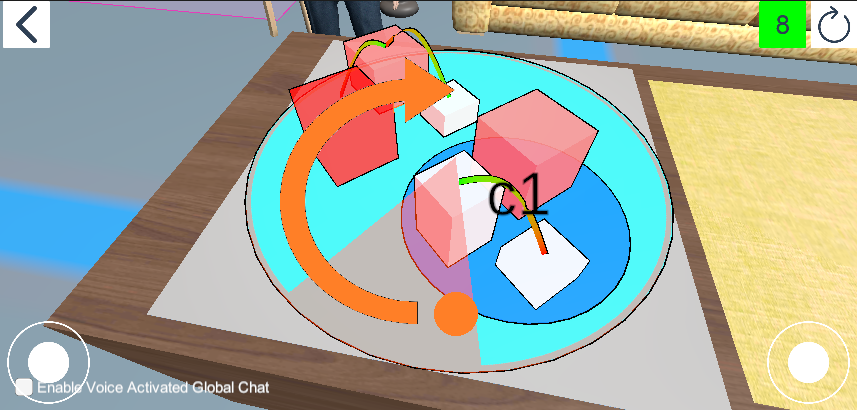
\includegraphics[width=1\textwidth]{Implementation/img/rotate.png}
    \caption{The \gls{city} can be rotated by for example touching the screen on the orange dot and dragging from there like the arrow indicates.}\label{fig:rotate}
\end{figure}

The implementation for the interaction of rotating is done in the following steps:
\begin{enumerate}
    \item Check if there is exactly one touch input on an object of the type \enquote{\gls{node}}.
    \item Check if the \enquote{8} button is active
    \item Calculate the new position of the \gls{city} just like in the desktop version of \gls{see}
\end{enumerate}
\subsubsection{Moving}
Last but not least, the player action of moving a \gls{city} or object has to be implemented to fulfill the requirements of [R7].
The user can touch a certain point on a \gls{city} and drag it to move it as visualized in figure \ref{fig:move}.
The same can be done with any \gls{node} or \gls{plane} by activating the \enquote{1} button.
Same as for the rotate-interaction, the user can also activate the \enquote{8} to move an object or city in one of eight predefined directions.
Also, by selecting the \enquote{1} or \enquote{8} button, it will turn green to indicate that it is active.

\begin{figure}[htb]
    \centering
    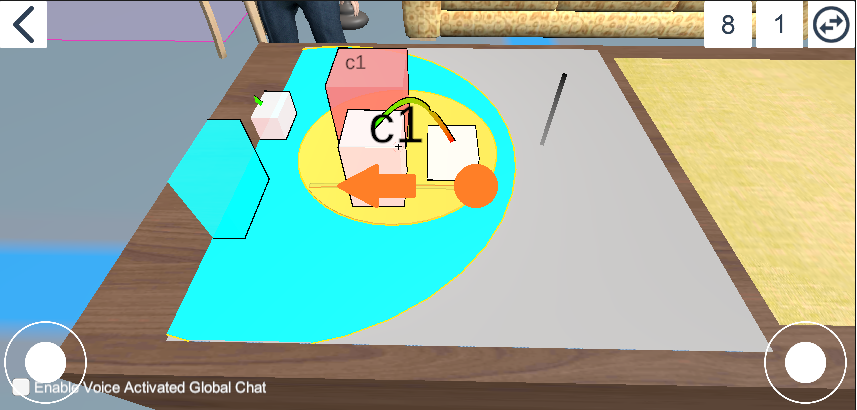
\includegraphics[width=1\textwidth]{Implementation/img/move.png}
    \caption{The \gls{city} can be moved by touching and dragging it to a desired direction.}\label{fig:left}
\end{figure}

The implementation is done similar to the one for the rotate-interaction. 
The only thing added here is the check whether the \enquote{1} button is active or not.

Note that for the rotate and move-interactions the \enquote{n} buttons have been removed (see figure \ref{fig:rotate_proto} and figure \ref{fig:move}).
This is because these buttons are not needed, since the initial mode, when entering the interaction, is already for the whole \gls{city}.
Also, the rotate object button and the rotate around selection center button have been removed. 
Rotating around a selection center will always be activated and can be deactivated by removing the selection of objects.
Rotating single objects is not intended as an interaction in \gls{see}.

\subsection{Android Build Requirements}
The last part of this chapter will discuss the requirements to build a version of \gls{see} on \gls{android} to fulfill the last requirement [R1].
In the following, there will be a deeper look at the challenges porting \gls{see} to \gls{android} devices brings. 


\subsubsection{Conditional Compilation}

\gls{see} uses, as it is usual, many \glspl{asset} for a medium to large \gls{unity} project.
Unfortunately, not all \glspl{asset} support an \gls{android} implementation.
Therefore, the unsupported assets have to be exchanged or excluded from the implementation.
Some unsupported \glspl{asset} are \textit{Valve} and \textit{UnityEngine.Windows.Speech}.
The \textit{Valve} \gls{asset} is required for the \gls{vr} implementation of \gls{see} and \textit{UnityEngine.Windows.Speech} is fundamental for the speech assistant \enquote{See}.
Since the \glspl{asset} are not supported but still needed in the project, they need to be excluded. 

Unity offers a way to compile only partial code. 
Therefore, it uses the \textit{directives}\footnote{https://docs.unity3d.com/Manual/PlatformDependentCompilation.html (last visited: 21.06.2022, 1:27)} of the C\# language. 
These use the hash character (\#) followed by \textit{if} or \textit{endif} to mark code areas with a condition.
\gls{unity} has platform scripting symbols like \textit{UNITY\_ANDROID} to set conditions for code areas to be compiled for a certain device or not.
The following code example shows how the technique is used in this project. 

\begin{minipage}{\linewidth}

\begin{lstlisting}[language=C]
using SupportedPackage
#if not UNITY_ANDROID
using NotSupportedForAndroidPackage
#endif 

    SomeClass
    {
    ...
    SomeSupportedPackageMethod()
    ...
    #if not UNITY_ANDROID
    SomeNotAvailableMethodForAndroid()
    #endif
    ...
    }
\end{lstlisting}

\end{minipage}

Examples like this can be found many times in the \gls{see} project. 
In addition to that, there are some cases where the main code is exchanged, whether the device is an \gls{android} or not.
For example the player actions discussed earlier in this chapter require touch input and can not use the hover effect of a mouse cursor on a mobile device.
Therefore, on mobile devices the touch input code will be used and on desktop devices the mouse hover code, but both code parts use the same methods and variables.
Having two separated classes would make up redundant code. 
In opposition, excessive use of conditional compilation makes it harder to maintain code because it might have to be adjusted at multiple points for a single change.
This way part of the code could easily be forgotten and lead to bugs.

\subsubsection{File Loading}
One last challenge for the mobile implementation of \gls{see} was how files are handled in the project.
\gls{see} uses specify file space for \gls{unity} called \textit{StreamingAssets}\footnote{https://docs.unity3d.com/Manual/StreamingAssets.html (last visited: 21.06.22, 2:47)} to store for example the various states of an Evolution-\gls{city}.
An Evolution-\gls{city} visualizes multiple states of development.
Only the first state is preloaded, the other states are stored in the \textit{StreamingAssets} and are loaded at runtime. 
The problem however is that an \gls{android} application is packed into a \gls{jar}.
Files inside a \gls{jar} cannot be obtained without further ado.
To achieve access to files that are not initially loaded, \textit{WebRequests}\footnote{https://docs.unity3d.com/ScriptReference/Networking.UnityWebRequest.html (last visited: 21.06.22, 3:13)} have to be used for an \gls{android} implementation. 
Therefore, once again the code needs to be divided and handled with conditional compilation.
This has to be done at every point in the code where files are obtained the common way with \textit{SystemIO} methods. 


\subsubsection{Restructuring}
\label{sec:restructure}
The disadvantage of conditional compilation is that it makes code harder to maintain as discussed earlier.
To minimize this disadvantage, it was thought of restructuring the entire project to only have conditional compilation at a core component of \gls{see}.

The concept idea was to restructure the project in a way that from a core component all the different versions get initialized and only in that core component conditional compilation gets used.
All components would have abstract super classes that could be easily supplemented with assets that are not available for all platforms.
The platform specific classes would then only be compiled for a certain platform build, since they are divided in the core class.

Unfortunately, \gls{see} is already entangled and a restructuring in the described way above would take a high effort.
\gls{see} already has many components that depend on another part of \gls{see}. 
These parts however also depend on other parts of \gls{see}. 
Restructuring and setting a new order for the parts of \gls{see} that support the idea of a core part of \gls{see} would take too much effort for this thesis and was therefore not implemented.